\documentclass[14pt, fleqn, xcolor={dvipsnames, table}]{beamer}
\usepackage[T2A]{fontenc}
\usepackage[utf8]{inputenc}
\usepackage[english,russian]{babel}
\usepackage{amssymb,amsfonts,amsmath,mathtext}
\usepackage{cite,enumerate,float,indentfirst}
\usepackage{cancel}
\usepackage{color}
\usepackage{hyperref}
\hypersetup{colorlinks,urlcolor=NavyBlue}

\usepackage{tikz}                   
\usetikzlibrary{shadows}

% \usepackage{enumitem}
% \setitemize{label=\usebeamerfont*{itemize item}%
%   \usebeamercolor[fg]{itemize item}
%   \usebeamertemplate{itemize item}}

\graphicspath{{images/}}

\usetheme{Boadilla}
\usecolortheme{seahorse}
\usefonttheme{serif}
\renewcommand{\CancelColor}{\color{red}}

\setbeamercolor{footline}{fg=Blue!50}
\setbeamertemplate{footline}{
  \leavevmode%
  \hbox{%
  \begin{beamercolorbox}[wd=.333333\paperwidth,ht=2.25ex,dp=1ex,center]{}%
    Амосов Федор, СПбГУ
  \end{beamercolorbox}%
  \begin{beamercolorbox}[wd=.333333\paperwidth,ht=2.25ex,dp=1ex,center]{}%
    Санкт-Петербург, 2014
  \end{beamercolorbox}%
  \begin{beamercolorbox}[wd=.333333\paperwidth,ht=2.25ex,dp=1ex,right]{}%
  Стр. \insertframenumber{} из \inserttotalframenumber \hspace*{2ex}
  \end{beamercolorbox}}%
  \vskip0pt%
}
\newcommand\indentdisplays[1]{%
     \everydisplay{\addtolength\displayindent{#1}%
     \addtolength\displaywidth{-#1}}}
\newcommand{\itemi}{\item[\checkmark]}

\title{Построение карты пылевых облаков\\\small{}}
\author[]{
    \small{
        Амосов Федор, СПбГУ\\
        ~\\
        Руководитель: Цветков Александр, СПбГУ
    }
}
\date{}

\begin{document}

    \begin{frame}
        \maketitle
        \small
    \end{frame}

    \section{Постановка задачи}  
		
		\begin{frame}
            Глава 1. Введение        
        \end{frame}		
		
        \begin{frame}{Постановка задачи}
            Дан звездный каталог с данными о
            \begin{itemize}
                \item положениях
                \item параллаксах
                \item фотометрии
                \item спектральных классах и классах светимости
            \end{itemize}  
            Задача
            \begin{itemize}
                \item Построить трехмерную карту пылевых облаков 
            \end{itemize}         
        \end{frame}
        
        \begin{frame}{Каталог}
            Звездный каталог с данными о
            \begin{itemize}
                \item положениях
                \item параллаксах
                \item фотометрии
                \item спектральных классах и классах светимости
            \end{itemize}  
            $\Longrightarrow$ каталог Hipparcos ($10^5$ звезд)
        \end{frame}
        
    \section{Определения}
        \begin{frame}{Покраснение}
            $$
                E_{B - V} = (B - V)_{obs} - (B - V)_{int}
            $$
            Пример на звезде HIP 44800
            \begin{itemize}
                \item У нее в каталоге $(B - V)_{obs} = 0.535^m$
                \item Класс F7V, поэтому$^*$ $(B - V)_{int} = 0.493^m$
                \item Покраснение $0.535^m - 0.493^m = 0.042^m$
                \item Между нами и звездой пыли на $0.042^m$
            \end{itemize}
        \end{frame}

    \section{Зависимость покраснения от расстояния}    
    
		\begin{frame}
            Глава 2. Построение панорамы пылевых облаков 
        \end{frame}		    
    
        \begin{frame}{Идеальная кривая покраснения}
            \begin{center}
                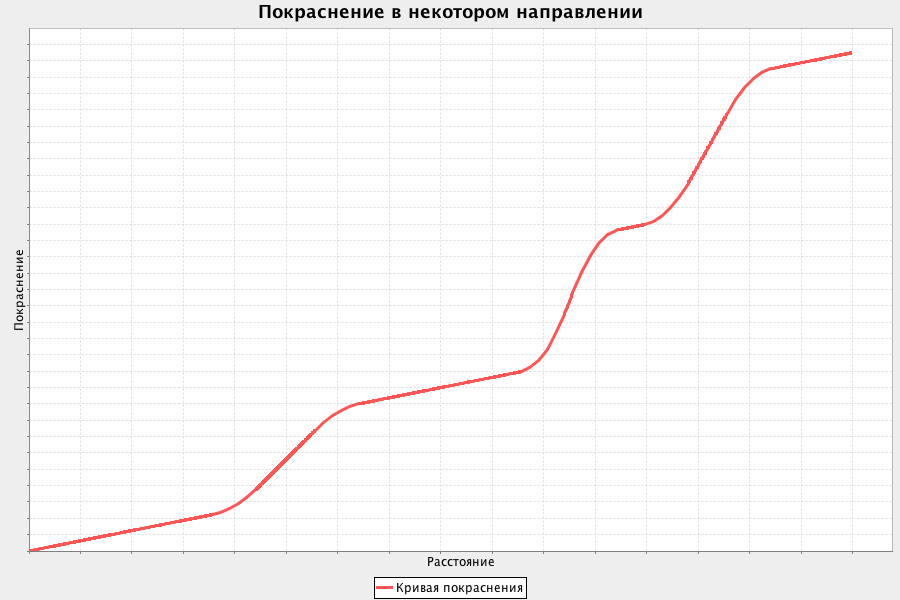
\includegraphics[scale=0.35]{ideal-1-no-tick.png}
            \end{center}             
        \end{frame}
        
        \begin{frame}{Пылевые облака}
            \begin{center}
                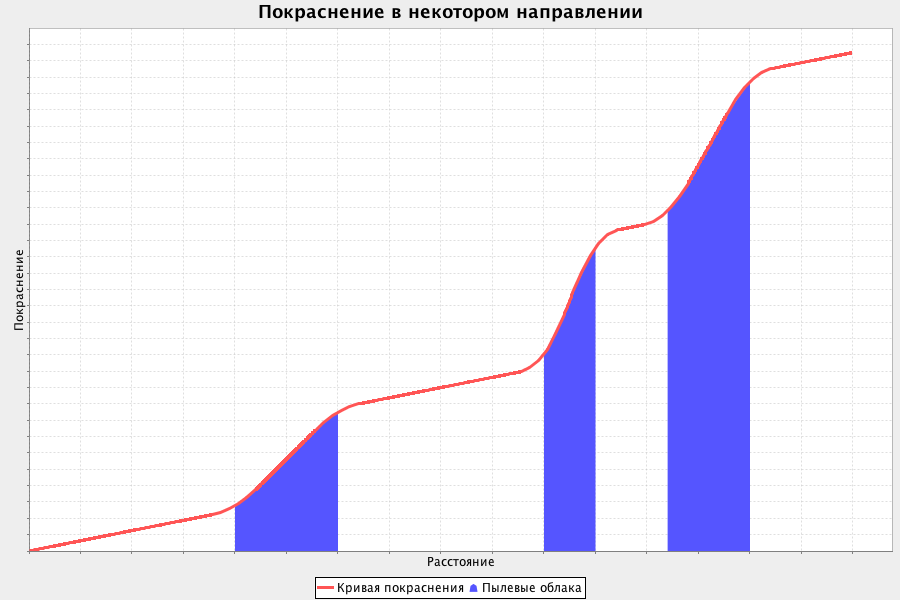
\includegraphics[scale=0.35]{ideal-2-no-tick.png}
            \end{center}             
        \end{frame}
        
        \begin{frame}{Реальное покраснение}
            \begin{center}
                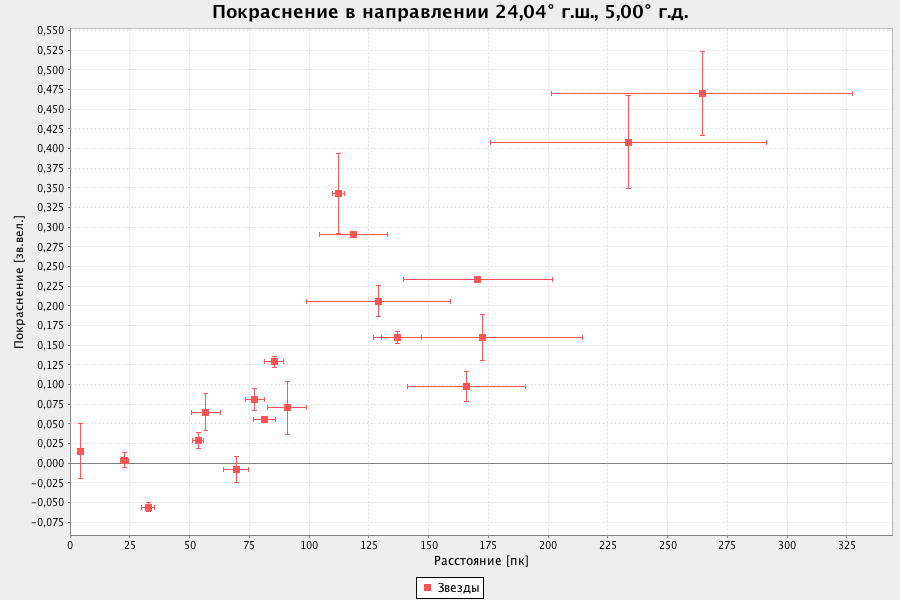
\includegraphics[scale=0.35]{real-1.png}
            \end{center}             
        \end{frame}
        
        \begin{frame}{Реальная <<кривая>> покраснения}
            \begin{center}
                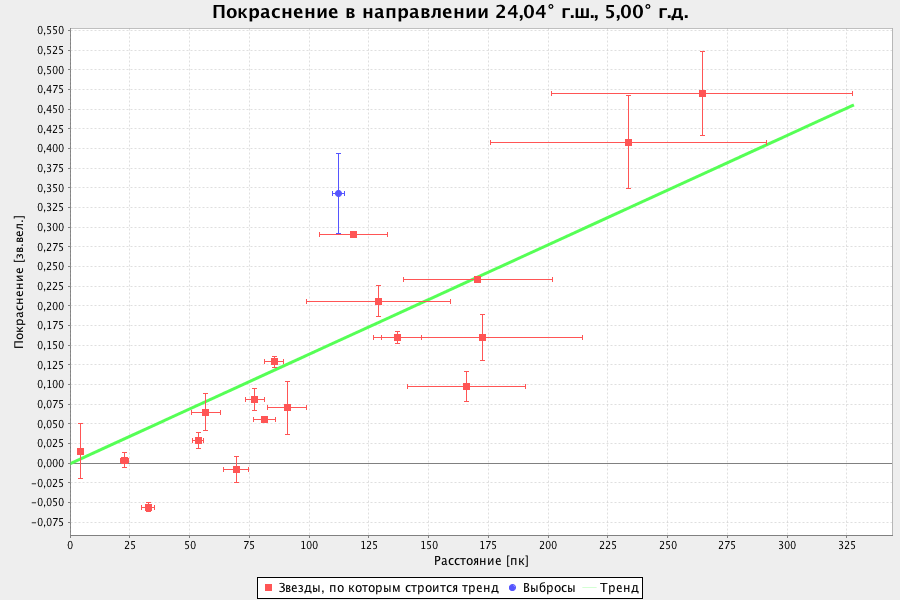
\includegraphics[scale=0.35]{real-2-k.png}
            \end{center}             
        \end{frame}
        
        \begin{frame}{<<В среднем>>}
            \begin{center}
                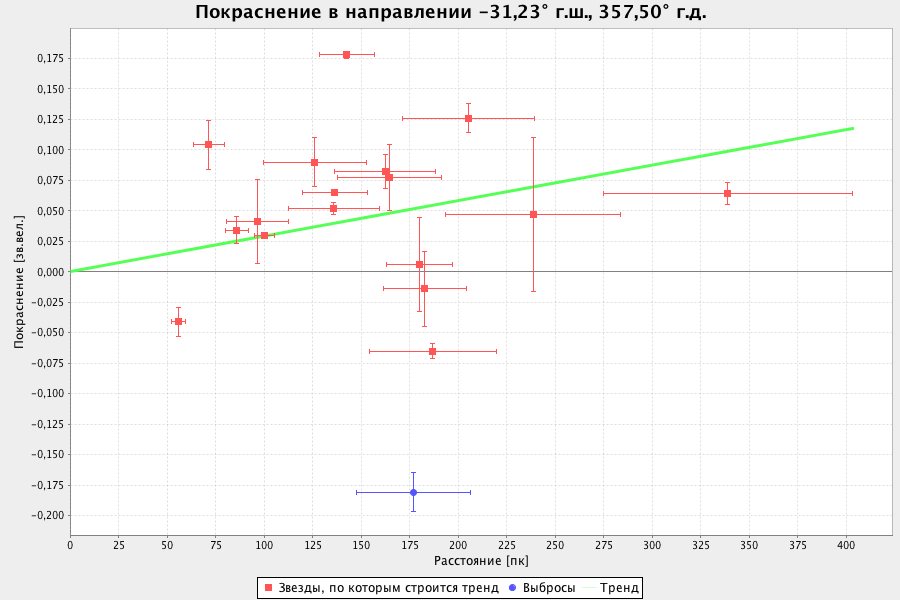
\includegraphics[scale=0.35]{real-3-k.png}
            \end{center}             
        \end{frame}        
        
        \begin{frame}{Отрицательный тренд}
            \begin{center}
                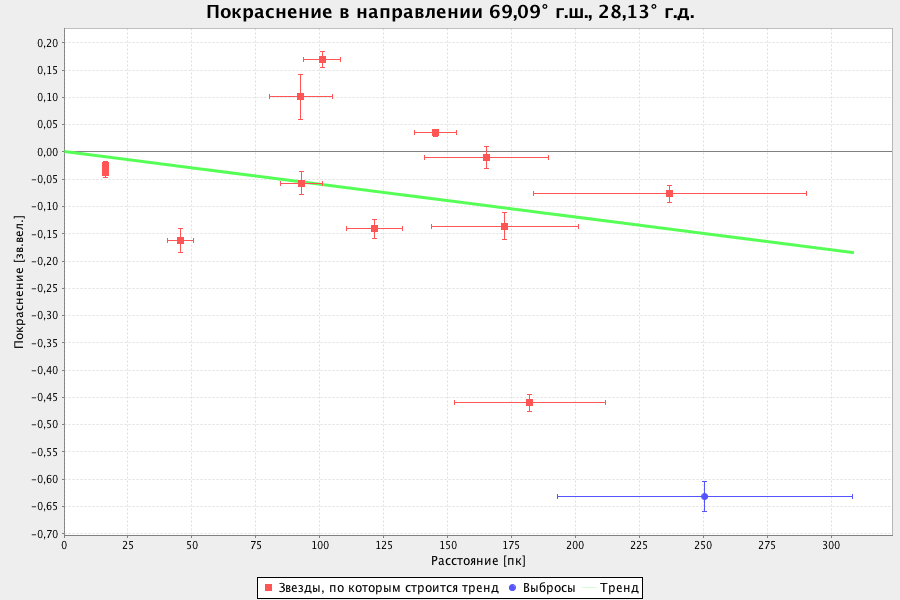
\includegraphics[scale=0.35]{real-4-k.png}
            \end{center}             
        \end{frame}
        
    \section{Карты}            
        
        \begin{frame}{Коэффициент $k$ ~~~~~~~~~~~~~~~~ $E_{B - V} = k r$}
            \begin{center}
                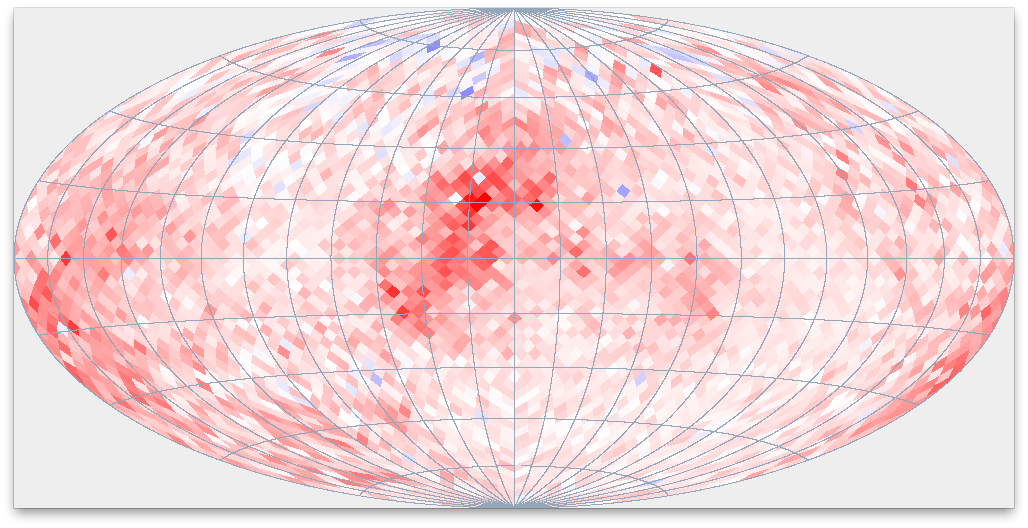
\includegraphics[scale=0.32]{map-k.png}
            \end{center}             
        \end{frame}
        
        \begin{frame}{Коэффициент $k$ с ошибкой}
            \begin{center}
                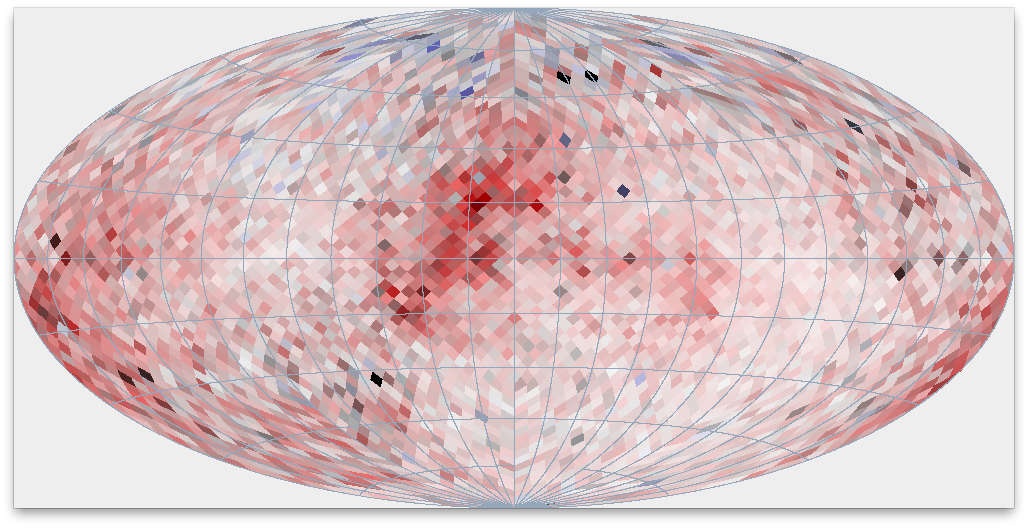
\includegraphics[scale=0.32]{map-k-sigma.png}
            \end{center}             
        \end{frame}
        

    \section{Предварительная обработка}                
        
        \begin{frame}{Предварительная обработка}
            \begin{itemize}
                \item В расчет берутся 58486 из 118219 звезд
                \begin{itemize}
                    \item Отсутствие некоторых необходимых данных$^*$
                    \item Точность в расстоянии 25\%
                \end{itemize}
                \item Разбиение сферы на $12 \cdot 18^2 = 3888$ равновеликих частей алгоритмом Healpix
                \item Тренды строятся по 90\% расчетных звезд
                \item Расчет отсутствующих классов светимости
                \begin{itemize}
                    \item Спектральный класс, класс светимости $\Longrightarrow (B - V)_{int}$
                \end{itemize}
            \end{itemize}
        \end{frame}
        
        \begin{frame}{Наличие классов светимости}
            \begin{center}
                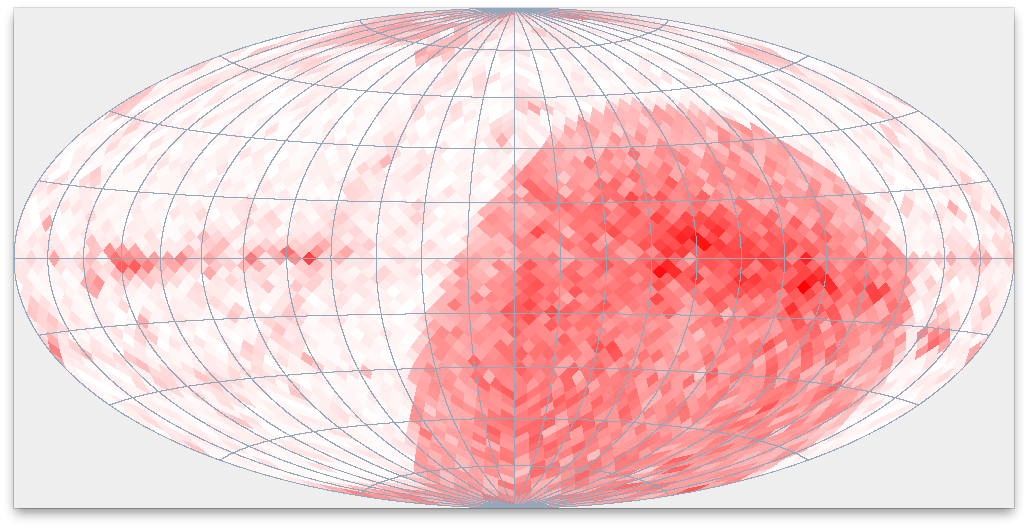
\includegraphics[scale=0.32]{count-white.png}
            \end{center}             
        \end{frame}

    \section{Определение классов светимости}                
        
        \begin{frame}{Обучение классификатора}
            \begin{center}
                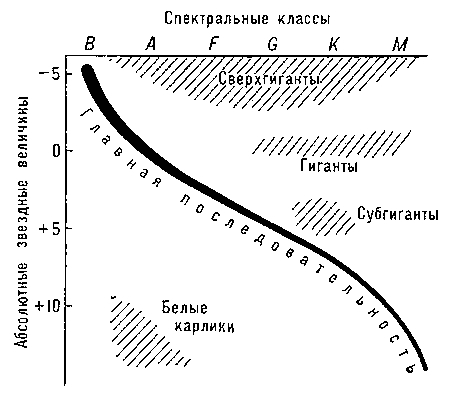
\includegraphics[scale=0.25]{gr-example.jpg}
            \end{center}
           
            \begin{itemize}
                \item Факторы: показатель цвета, абсолютная звездная величина
                \item Класс: класс светимости
                \item Алгоритм классификации: метод опорных векторов (Support Vector Machines, SVM)
            \end{itemize}
        \end{frame}        
        
        \begin{frame}{Обучающее множество}
            \begin{center}
                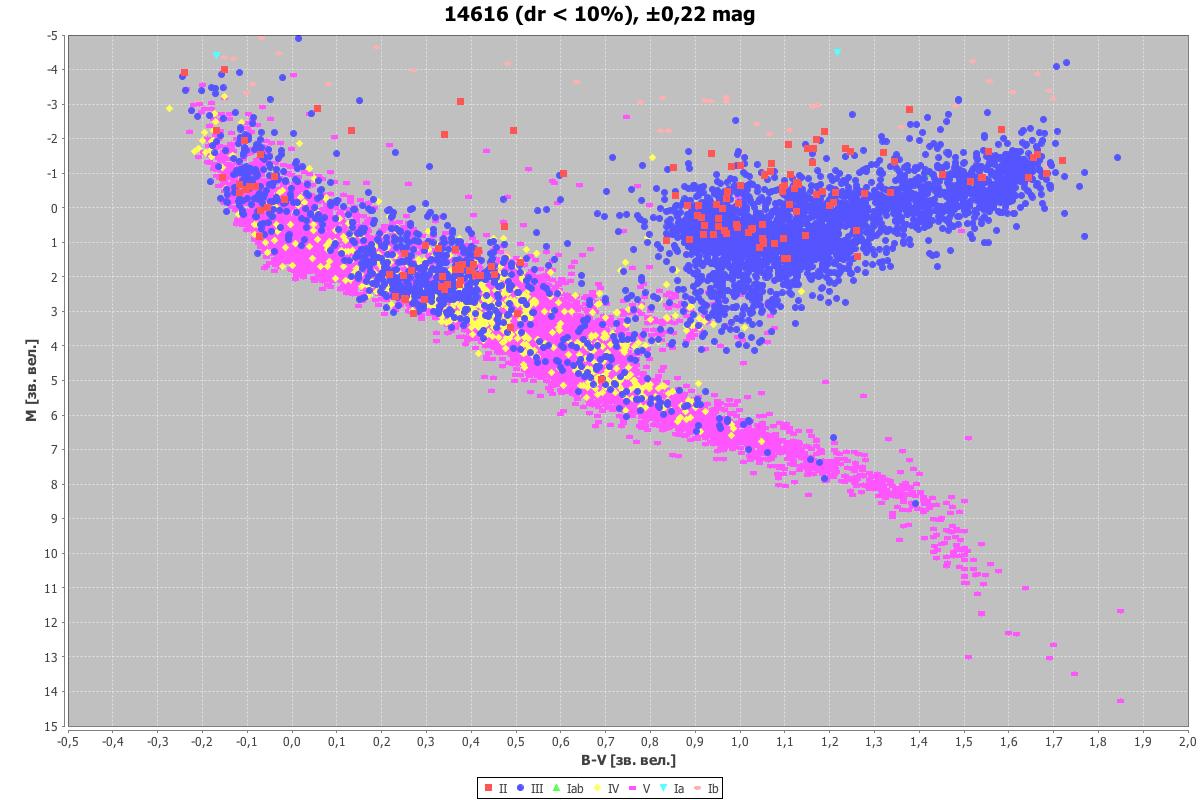
\includegraphics[scale=0.25]{ml-1.png}
            \end{center}             
        \end{frame}
        
        \begin{frame}{Результат классификации}
            \begin{center}
                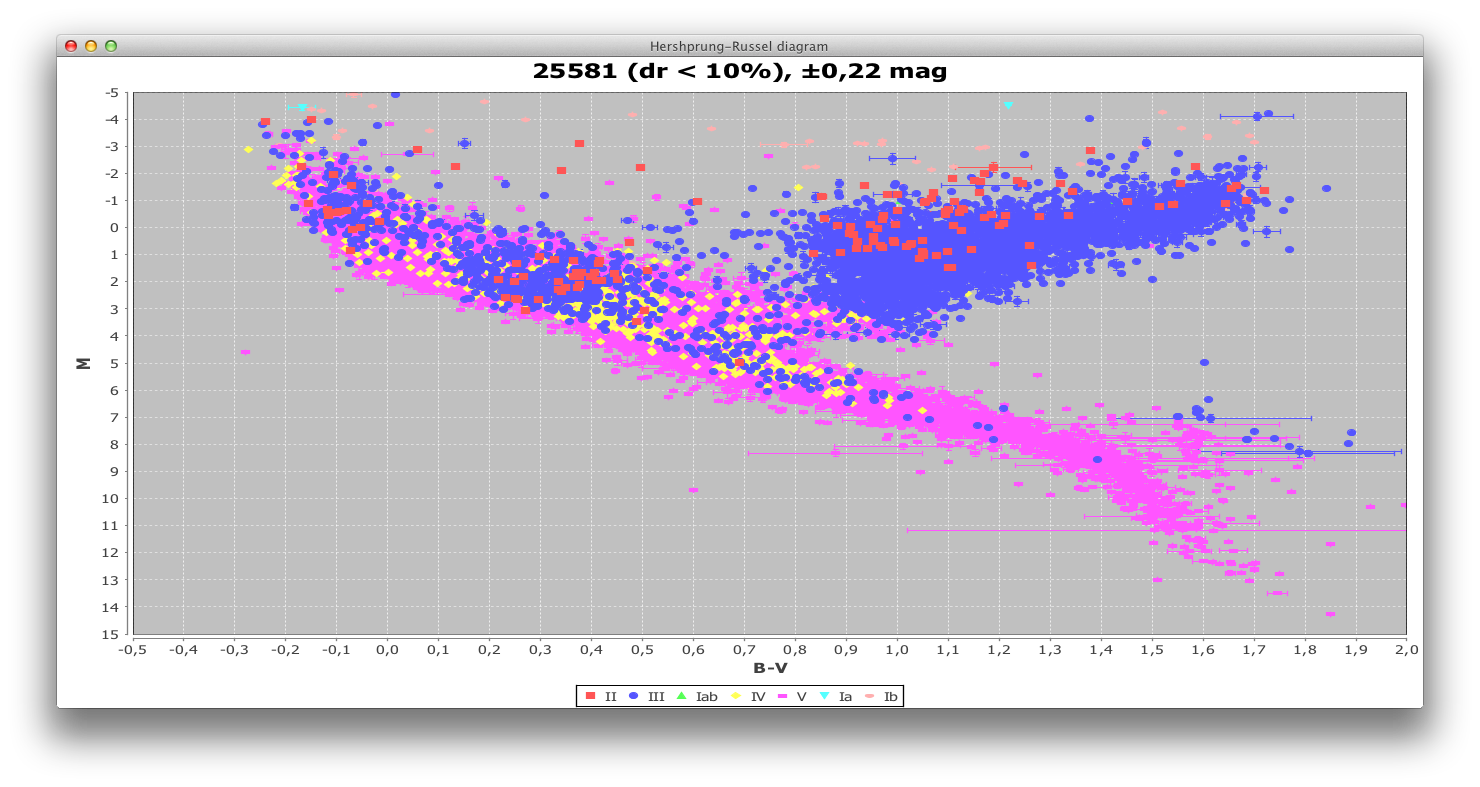
\includegraphics[scale=0.25]{ml-2.png}
            \end{center}             
        \end{frame}
        
        \begin{frame}{Качество классификации}
            Результаты кросс--валидации на 10 частях
            \begin{itemize}
                \item Точность 93.4\%
                \item Полнота 93.0\%
                \item F--мера 92.7\%
            \end{itemize}
            Замечание
            \begin{itemize}
                \item Обучение проводилось только на III и V классах
            \end{itemize}
        \end{frame}                  
        
        \begin{frame}{Результат}
            \begin{center}
                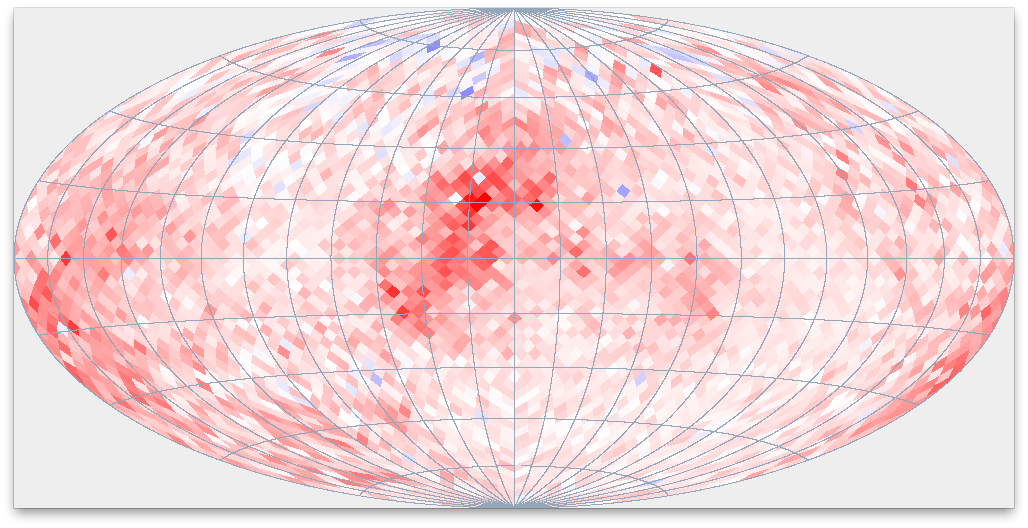
\includegraphics[scale=0.32]{map-k.png}
            \end{center}             
        \end{frame}
        
        \begin{frame}{Что дальше?}
            \begin{center}
                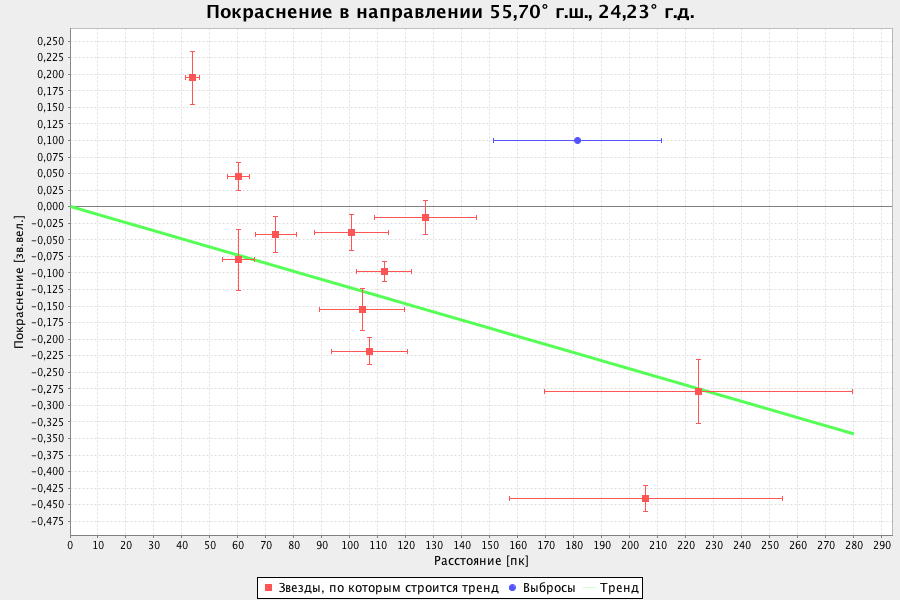
\includegraphics[scale=0.3]{next-k.png}
            \end{center}  
            $$E_{B - V} + 3 \sigma_{E_{B - V}} < 0$$
        \end{frame} 
        
	
	 \section{Отрицательное покраснение}          
        
        \begin{frame}
            Глава 3. Звезды каталога Hipparcos с отрицательным покраснением 
        \end{frame}		    
        
        \begin{frame}{Выбросы на небе}
            \begin{center}
                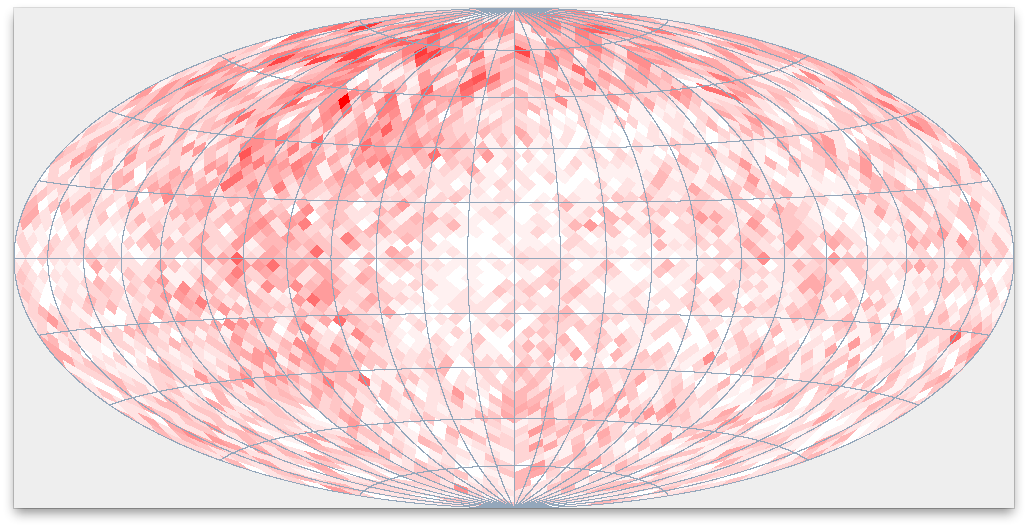
\includegraphics[scale=0.32]{outlier-map.png}
            \end{center}             
        \end{frame}   
        
        \begin{frame}{Выбросы и параллакс}
            \begin{center}
                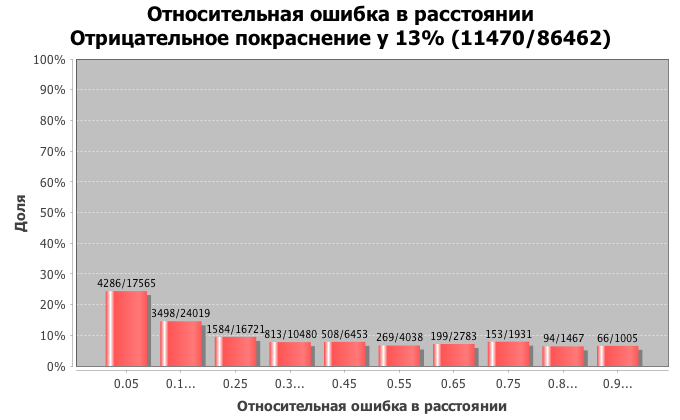
\includegraphics[scale=0.49]{outlier-r.png}
            \end{center}             
        \end{frame}     
        
        \begin{frame}{Выбросы и показатель цвета}
            \begin{center}
                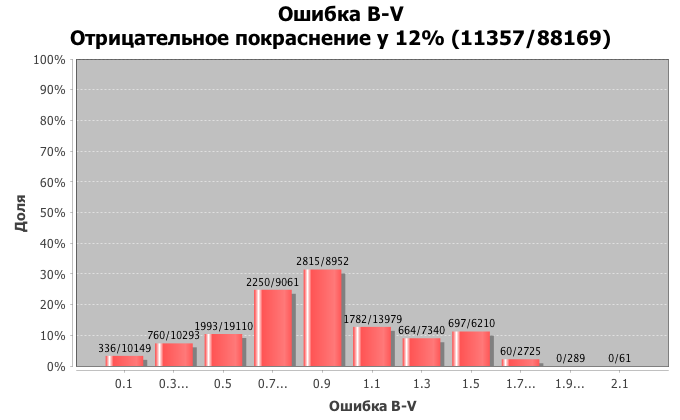
\includegraphics[scale=0.49]{outlier-bv.png}
            \end{center}             
        \end{frame}   
        
        \begin{frame}{Выбросы и спектр}
            \begin{center}
                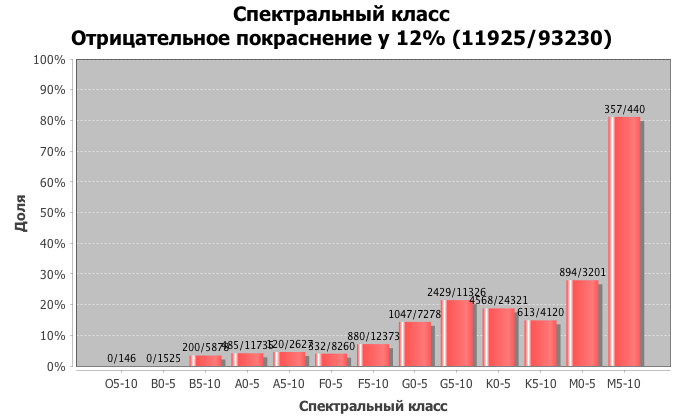
\includegraphics[scale=0.49]{outlier-spect.png}
            \end{center}             
        \end{frame}  
        
        \begin{frame}{Выбросы и спектр (III)}
            \begin{center}
                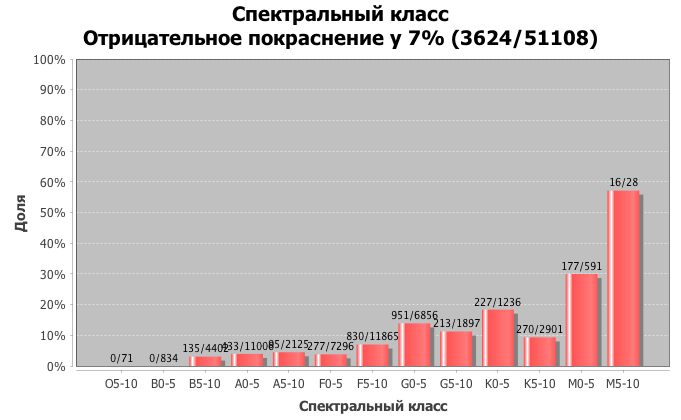
\includegraphics[scale=0.49]{outlier-spectIII.png}
            \end{center}             
        \end{frame} 
        
        \begin{frame}{Выбросы и спектр (V)}
            \begin{center}
                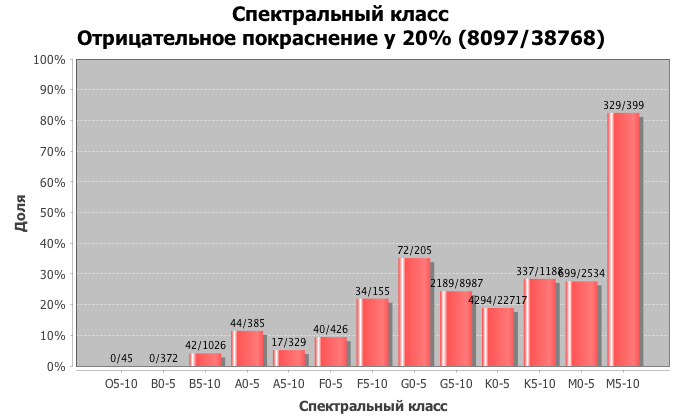
\includegraphics[scale=0.49]{outlier-spectV.png}
            \end{center}             
        \end{frame} 
        
		\begin{frame}{Выброы и диаграмма ГР}
            \begin{center}
                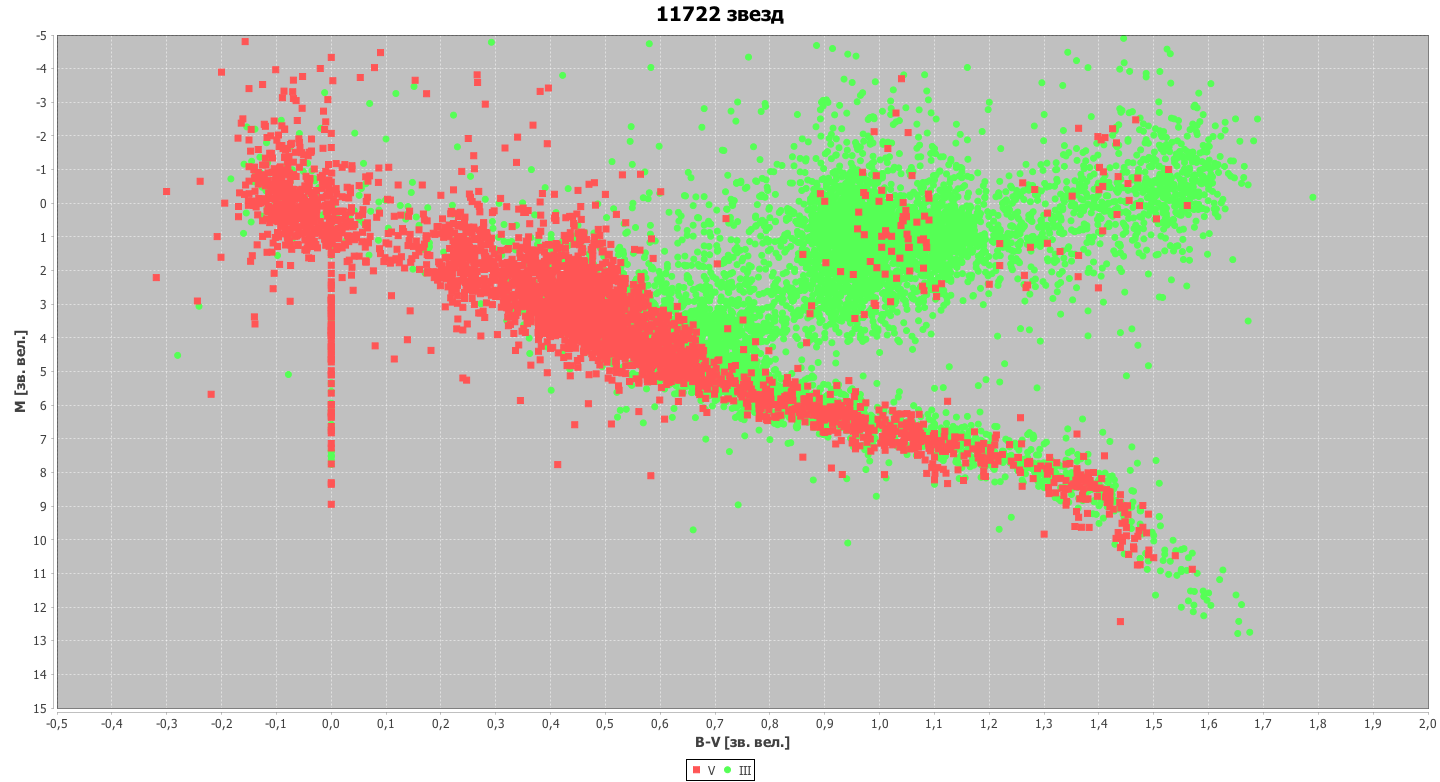
\includegraphics[scale=0.2]{outlier-hr.png}
            \end{center}    
            $$(B - V)_{int}(III)  > (B - V)_{int}(V)$$
            $$E_{B - V} = (B - V)_{obs} - (B - V)_{int}$$        
        \end{frame}         
        
        \begin{frame}{Таблица (Цветков)}
            \begin{center}
                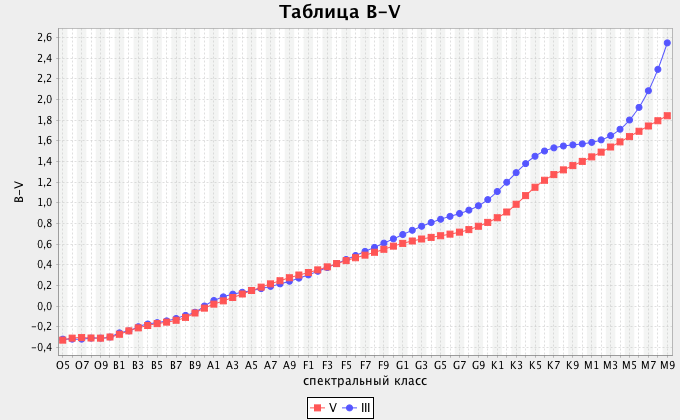
\includegraphics[scale=0.45]{table-tsvetkov.png}
            \end{center} 
            \tiny{Неточности в спектальной классификации звезд каталога Tycho-2 Spectral Type
А.А.Сминов, А.С.Цветков, А.В.Попов
2006}
        \end{frame} 
        
        \begin{frame}{Таблица (Schmidt-Kaler)}
            \begin{center}
                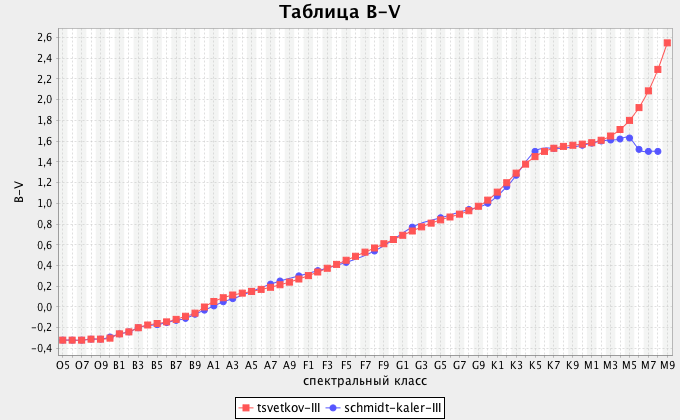
\includegraphics[scale=0.49]{table-sk.png}
            \end{center}
        \end{frame} 
        
        \begin{frame}{Расчет верхней оценки}
            \begin{itemize}
            		\item Дан порог (к примеру, 5\%)
            		\item Для каждого класса светимости и спектрального класса рассмотрим все звезды этих классов
            		\item Отсортируем их по $E_{B - V} + 3 \sigma_{E_{B - V}}$
            		\item Рассмотрим звезду, соответствующую порогу
            			$$E_{B - V} + 3 \sigma_{E_{B - V}} = E ~~ (< 0)$$
            			$$(B - V)_{obs} - (B - V)_{int} + 3 \sigma_{(B - V)_{obs}} = E$$
            			$$(B - V)_{obs} - (B - V)^{max}_{int} + 3 \sigma_{(B - V)_{obs}} = 0$$
            		\item $(B - V)^{max}_{int} = (B - V)_{obs} + 3 \sigma_{(B - V)_{obs}}$
            \end{itemize}
           
        \end{frame} 
        
        \begin{frame}{Верхняя оценка}
            \begin{center}
                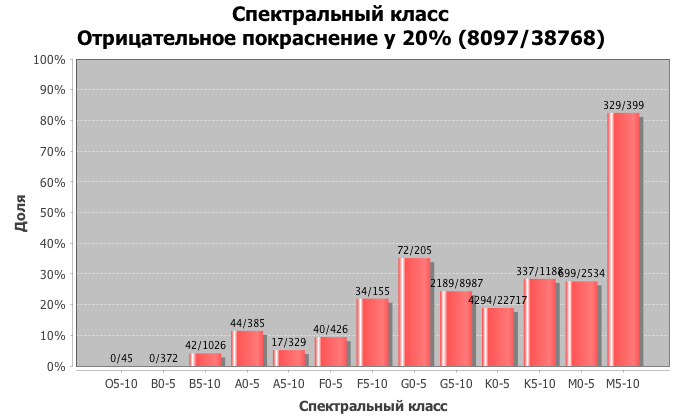
\includegraphics[scale=0.24]{outlier-spectV.png}
			    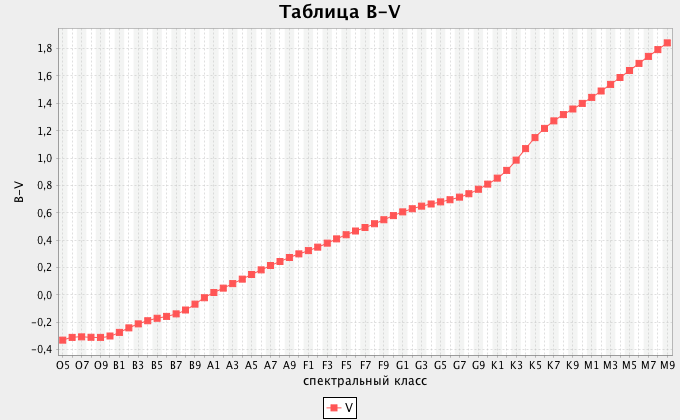
\includegraphics[scale=0.24]{table-tsvetkovV.png}
                                
            \end{center}
            \begin{center}
                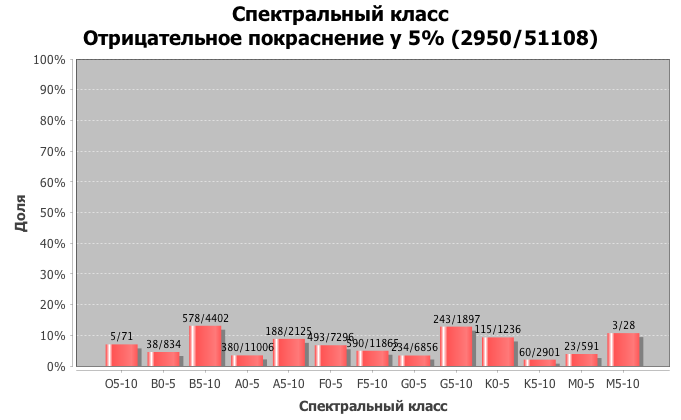
\includegraphics[scale=0.24]{outlier-max5.png}
			    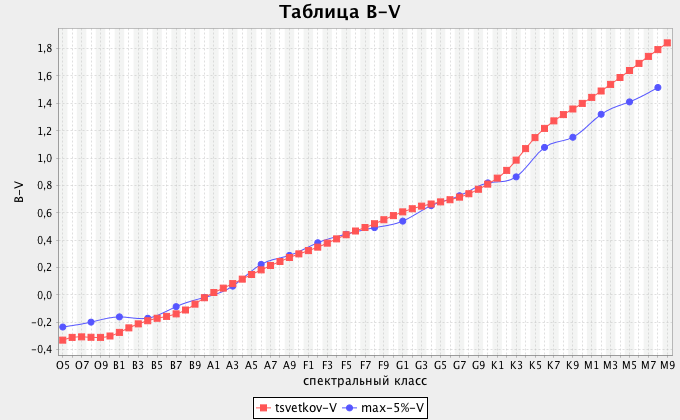
\includegraphics[scale=0.24]{table-max5.png}
                                
            \end{center}
        \end{frame} 
        
        \begin{frame}{Верхняя оценка}
            \begin{center}
			    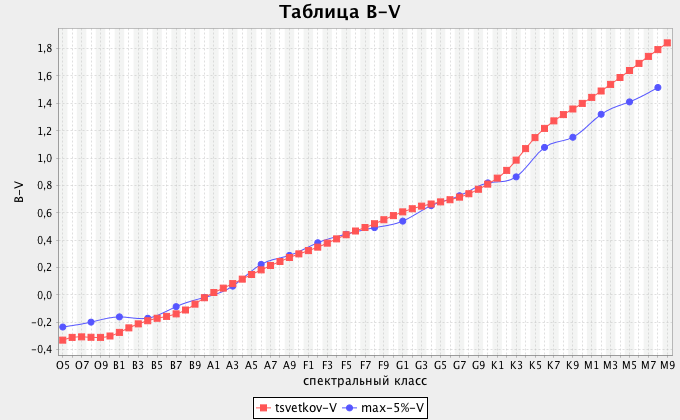
\includegraphics[scale=0.49]{table-max5.png}
            \end{center}
        \end{frame} 
        
        \begin{frame}{Новая таблица (V)}
            \begin{center}
			    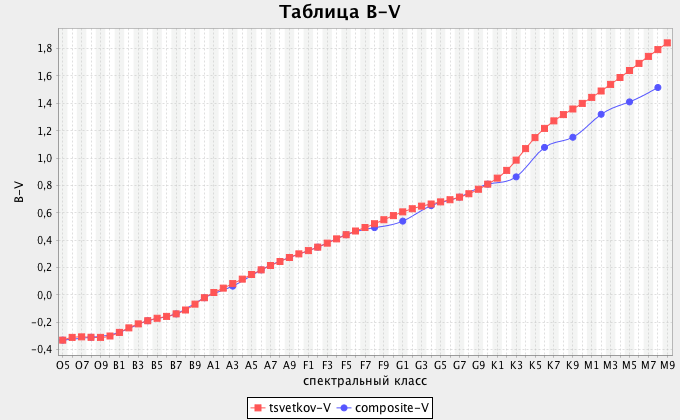
\includegraphics[scale=0.49]{table-compositeV.png}
            \end{center}
        \end{frame} 
        
        \begin{frame}{Новая таблица (III)}
            \begin{center}
			    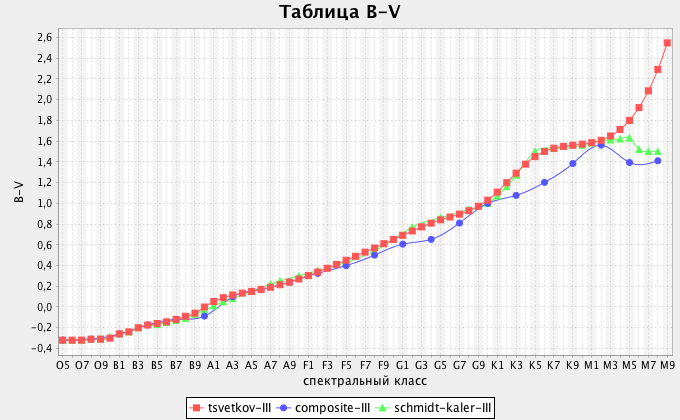
\includegraphics[scale=0.49]{table-compositeIII.png}
            \end{center}
        \end{frame} 
        
    \section{Построение трехмерной карты пылевых облаков}          
        
		\begin{frame}
            Глава 4. Построение трехмерной карты пылевых облаков 
        \end{frame}	
        
        \begin{frame}{Есть ли пыль в точке?}
            \begin{center}
                
\includegraphics[scale=1.6]{dust.jpg}
            \end{center}
        \end{frame} 
        
         \begin{frame}{Алгоритм поиска пыли}
            \begin{itemize}
            		\item Бросаем много точек с распределением, соответствующем распределению звезд. \\ Для каждой:
            		\item Находим $K$ ближайших звезд. Проверяем локальность полученной окрестности.
            		\item Вычисляем тренд $a r + b$ покраснения по этим звездам
            		\item Если $a > threshold$, то в точке есть пыль
            \end{itemize}
        \end{frame} 
        
        
        \begin{frame}{Алгоритм поиска пыли. Реализация}
            \begin{itemize}
            		\item Берем звезды с относительной ошибкой в расстоянии $\le 35\% \longrightarrow 64176$ звезд
            		\item Бросаем $10^6$ точек
            		\item $K = 25$
            		\item Используем KD-деревья для поиска ближайших соседей. Поиск за $O(\log n)$
            		\item Диаметр окрестности $\le 200$ пк
            		\item $threshold =  0.008$ зв.вел./пк
            \end{itemize}
        \end{frame} 
        
        \begin{frame}{<<Трехмерная>> карта пыли}
            \begin{center}
                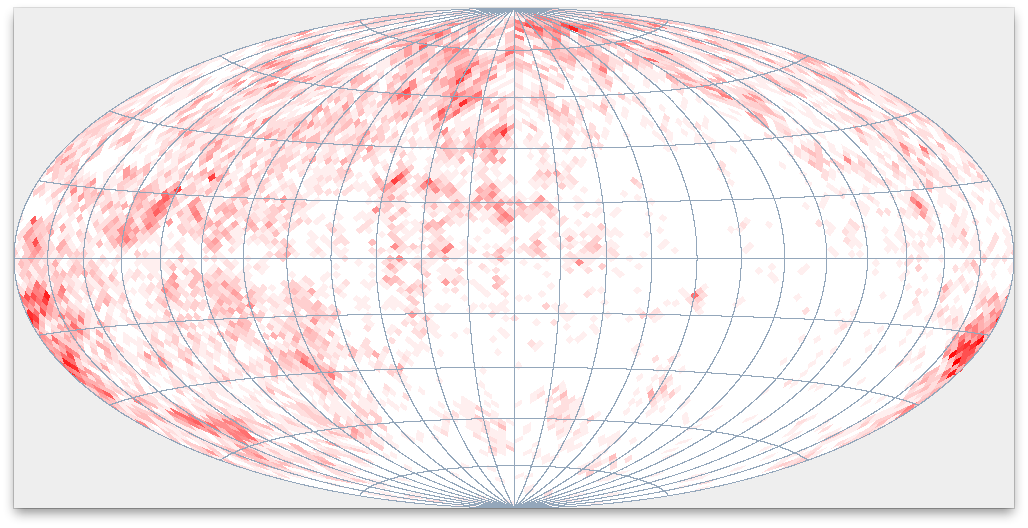
\includegraphics[scale=0.32]{dust-3d.png}
            \end{center}             
        \end{frame}   
        
        \begin{frame}{Собрираем из пыли облака}
            \begin{itemize}
            		\item 12560 точек пыли
            		\item Кластеризация методом DBSCAN за $O(n \log n)$
            		\item Центр облака - центр масс точек кластера
            		\item Радиус облака - усредненное стандартное отклонение точек кластера по $x, y, z$
			\end{itemize}                   
        \end{frame}   
        
        \begin{frame}{Пылевые облака}
            \begin{center}
                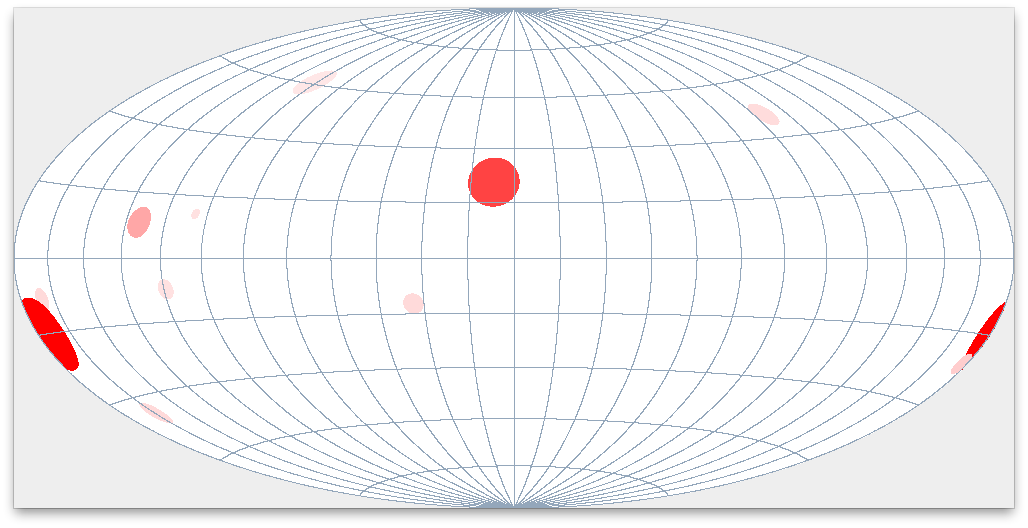
\includegraphics[scale=0.32]{clouds-3d.png}
            \end{center}             
        \end{frame}  
        
	\section{Результаты}            
        
        \begin{frame}
            Глава 5. Результаты
        \end{frame}	
        
        \begin{frame}{Основные результаты}
            \begin{itemize}
            		\item Построена панорама пыли
            		\item Разработан алгоритм поиска пыли
            		\item Построена трехмерная карта пыли
            		\item Найдены облака
            			
			\end{itemize}     
			\begin{center}
            		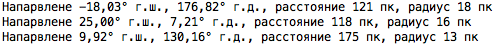
\includegraphics[scale=0.6]{clouds.png}
            	\end{center}                 
        \end{frame} 
        
        \begin{frame}{Вспомогательные результаты}
            \begin{itemize}
            		\item Найдены недостающие классы светимости спомощью классификатора
            		\item Представлена попытка найти причину отрицательного покраснения у  звезд
            		\item Получена верхняя оценка на показатель цвета в таблицах
            		\item Разработана библиотека для работы с каталогом 
			\end{itemize}                      
        \end{frame} 
        
        \begin{frame}{Q\&A}
            \begin{center}
                Спасибо за внимание!\\
                \href{https://github.com/amosov-f/dust-detection}{github.com/amosov-f/dust-detection}
            \end{center}
        \end{frame}

\end{document}